\section{Trigger}
\label{sec:Trigger}

Due to the presence of four fully reconstructed leptons in the final state, the data events and detector-level MC events are preselected using a logical OR of different single and double-lepton triggers. The trigger menu varies according to the data-taking run periods to reflect the changes in the high-level trigger system, which are required to cope with increasing data rates. Additionally, trigger matching is required for the selected events. The trigger matching selects a subset of preselected events in which at least one lepton of the quadruplet is matched to one of the fired triggers. Table \ref{tab:Trigger} shows the trigger menu used by the analysis per different data periods using either electrons, muons, or mixed electron-muon triggers. The \textit{HLT\_*} string specifies the high-level trigger menu used where the "e" or "mu" substring specifies the type of object used to fire the trigger, and the attached number specifies the minimum $p_{T}$ threshold for the object. The substring \textit{lh*} attached to \textit{HLT\_*} stands for the likelihood identification working point for the electrons, and the \textit{ivar*} specifies the isolation working point used for either object. The string \textit{L1*} indicates the use of either calorimeters or MS L1 trigger, and the string \textit{noL1} suggests the absence of L1 triggers. 

\begin{table}[!htbp]
    \centering
    \begin{tabular}{| l | c | c |}
    \hline 
    Period & Leptons & Triggers \\
    \hline
    \multirow{10}{*} {2015} & \multirow{4}{*} {Electron} &  HLT$\_$e24$\_$lhmedium$\_$L1EM20VH  \\
                        &          &  HLT$\_$e60$\_$lhmedium \\
                        &    & HLT$\_$e120$\_$lhloose \\
                        & &  HLT$\_$2e12$\_$lhvloose$\_$L12EM10VH\\\cline{2-3}

                        & \multirow{4}{*} {Muon} & HLT$\_$mu20$\_$iloose$\_$L1MU15 \\
                        & & HLT$\_$mu50 \\
                        & & HLT$\_$2mu10 \\
                        & & HLT$\_$mu18$\_$mu8noL1 \\\cline{2-3}
                        & \multirow{2}{*}{Mixed} & HLT$\_$e7$\_$lhmedium$\_$mu24 \\
                        & & HLT$\_$e17$\_$lhloose$\_$mu14 \\
    \hline
    \multirow{10}{*} {2016} & \multirow{4}{*} {Electron} & HLT$\_$e26$\_$lhtight$\_$nod0$\_$ivarloose \\
                        &          & HLT$\_$e60$\_$lhmedium$\_$nod0 \\
                        & & HLT$\_$e140$\_$lhloose$\_$nod0\\
                        & &  HLT$\_$2e17$\_$lhvloose$\_$nod0 \\\cline{2-3}
                        & \multirow{4}{*} {Muon} & HLT$\_$mu26$\_$ivarmedium \\
                        & & HLT$\_$mu50 \\
                        & & HLT$\_$2mu14 \\
                        & & HLT$\_$mu22$\_$mu8noL1 \\\cline{2-3}
                        & \multirow{2}{*}{Mixed} & HLT$\_$e7$\_$lhmedium$\_$nod0$\_$mu24  \\
                        & & HLT$\_$e17$\_$lhloose$\_$nod0$\_$mu14 \\
    \hline
    \multirow{10}{*} {2017} & \multirow{4}{*} {Electron} &  HLT$\_$e26$\_$lhtight$\_$nod0$\_$ivarloose \\
                        & &  HLT$\_$e60$\_$lhmedium$\_$nod0 \\
                        & & HLT$\_$e140$\_$lhloose$\_$nod0 \\
                        &          & HLT$\_$2e24$\_$lhvloose$\_$nod0 \\\cline{2-3}
                        & \multirow{4}{*} {Muon} & HLT$\_$mu26$\_$ivarmedium \\
                        & & HLT$\_$mu50 \\
                        & & HLT$\_$2mu14 \\
                        & & HLT$\_$mu22$\_$mu8noL1  \\\cline{2-3}
                        & \multirow{2}{*}{Mixed} &  HLT$\_$e17$\_$lhloose$\_$nod0$\_$mu14  \\
                        & & HLT$\_$e26$\_$lhmedium$\_$nod0$\_$mu8noL1 \\
    \hline
    \multirow{10}{*} {2018} & \multirow{4}{*} {Electron} & HLT$\_$e26$\_$lhtight$\_$nod0$\_$ivarloose \\
                        &          & HLT$\_$e60$\_$lhmedium$\_$nod0  \\
                        &          & HLT$\_$e140$\_$lhloose$\_$nod0 \\
                        &          &  HLT$\_$2e24$\_$lhvloose$\_$nod0 \\\cline{2-3}
                        & \multirow{4}{*} {Muon} & HLT$\_$mu26$\_$ivarmedium \\
                        & & HLT$\_$mu50  \\
                        & & HLT$\_$2mu14 \\
                        & &  HLT$\_$mu22$\_$mu8noL1 \\\cline{2-3}
                        & \multirow{2}{*}{Mixed} & HLT$\_$e17$\_$lhloose$\_$nod0$\_$mu14 \\
                        & &  HLT$\_$e26$\_$lhmedium$\_$nod0$\_$mu8noL1  \\
    \hline
    \end{tabular}
    \caption{Trigger menu used in the analysis for event preselection \label{tab:Trigger}}
\end{table}

%The trigger efficiency of MC is defined as a ratio of events passing the logical OR selection of the triggers to the number of events passing reconstruction level pre-trigger selection. The trigger efficiency for MC events could differ from that for the data. Thus, trigger efficiency scale factors are applied to MC events to account for the differences. The scale factors are defined as a fraction of trigger efficiency for MC to that of data and retrieved from the ATLAS supported tool \textit{TrigGlobalEffciencyCorrectionTool}\footnote{https://gitlab.cern.ch/atlas/athena/tree/21.2/Trigger/TrigAnalysis/TrigGlobalEfficiencyCorrection}.

Figure \ref{fig:Trigger} shows the efficiency of trigger selection in events with a signal quadruplet and a dijet as a function of invariant mass of the four-lepton system ($m_{4\ell}$) in data and total SM prediction for $2015$-$2016$ data-taking period. The trigger efficiency is the ratio of events passing detector-level event selection and trigger requirements to the total number of events passing detector-level event selection requirements. For both data and prediction, the trigger efficiency is $100\%$. The requirements for detector-level event selection are discussed in Section \ref{sec:EventSel}.

\begin{figure}[!htb]
    \centering
    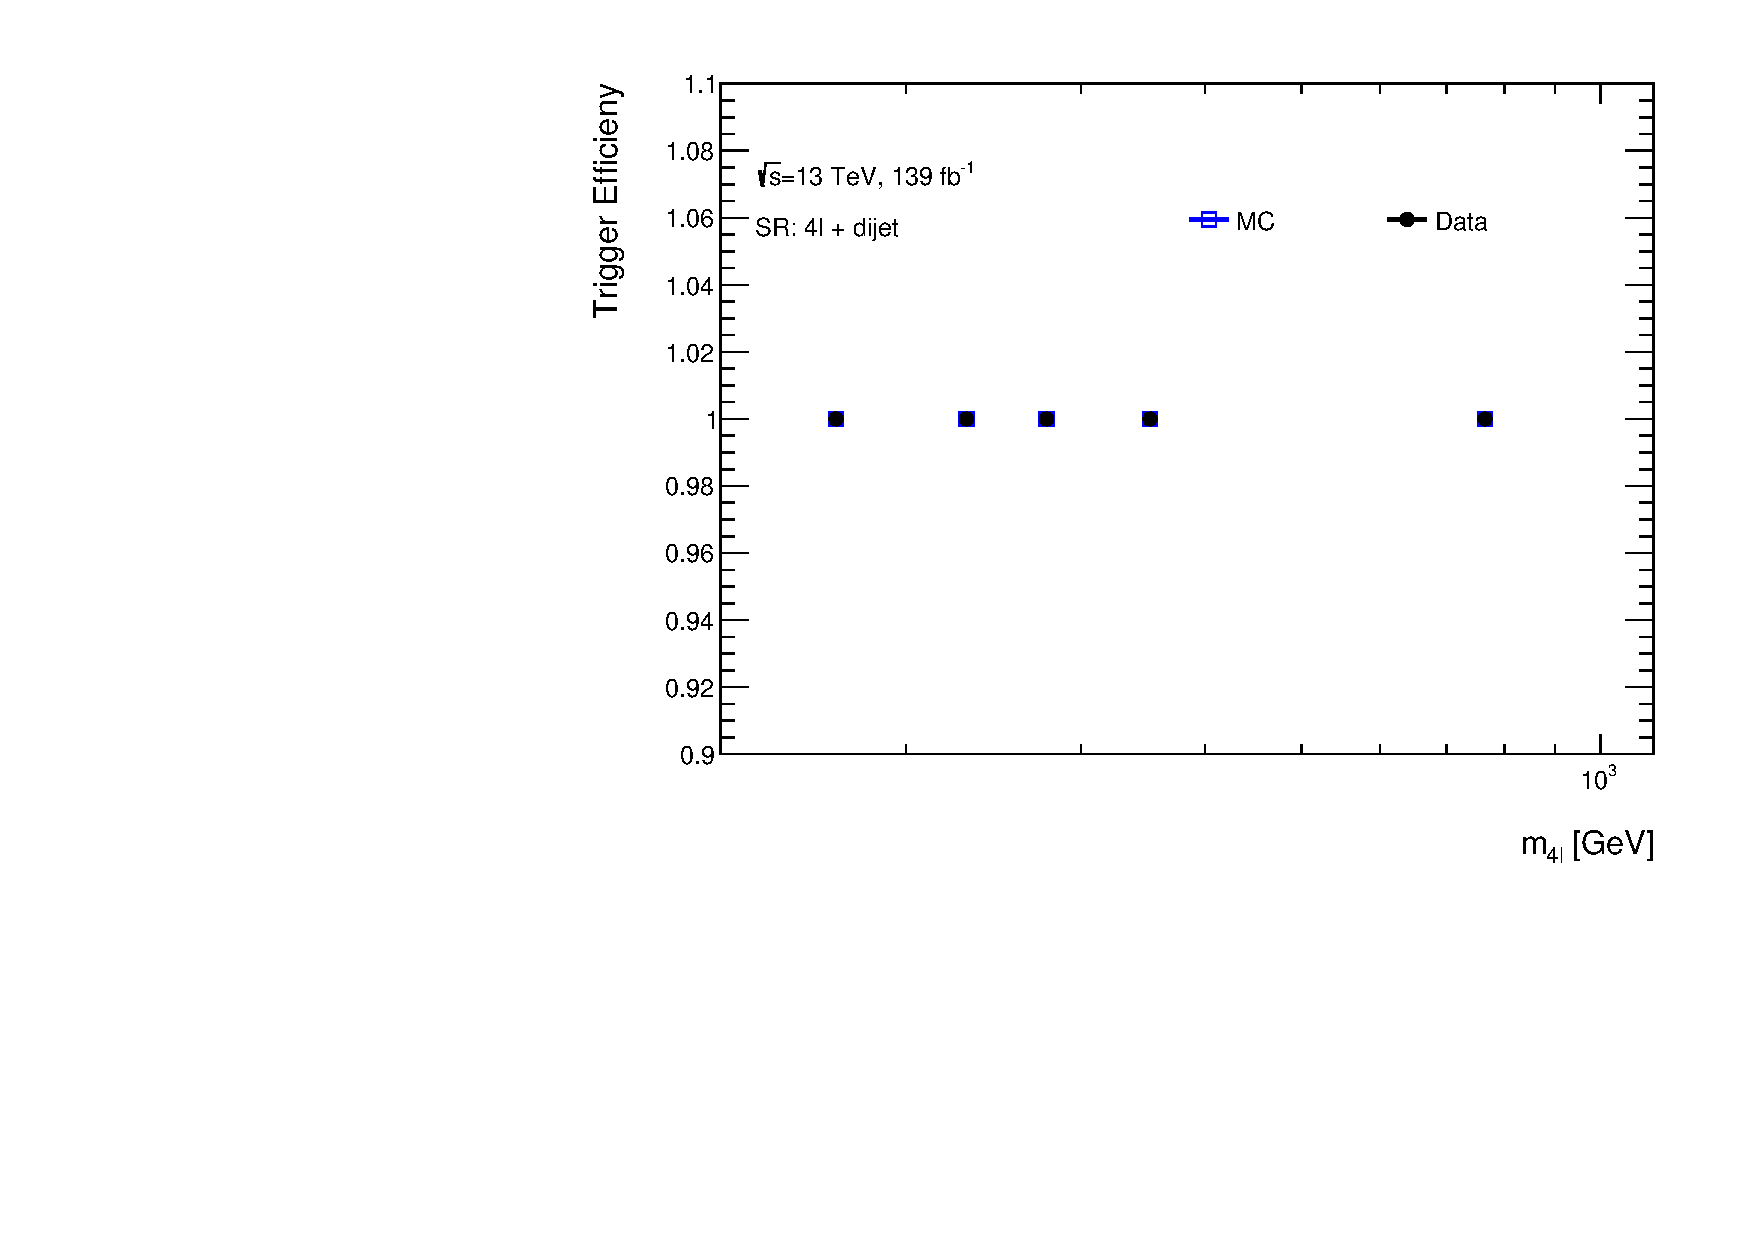
\includegraphics[width=.8\linewidth]{figures/AnalysisOverview/TriggerEfficiency_DataMC.pdf}
    \caption{ Trigger efficiency as a function of $m_{4\ell}$ in events with a quadruplet and a dijet in data and SM prediction corresponding to the $2015$-$2016$ data-taking period.\label{fig:Trigger}}
\end{figure}